\section*{Problem 2}
	Before the start, it is important that understanding \textit{Ramsey numbers}. This is based on \textit{Complete graph with n nodes}: $K_n$. The concept(definition) of $K_n$ is very easy, so I recommend looking it up and understanding it on Wikipedia($K_n$ is used after mid-term).\\
	$R(m, n) = r$ means:
	\begin{itemize}
		\item [] Initial setting: Edges of $K_r$ has only 2 colors: red or blue.\\
		For this $K_r$, we can find a $K_m$ subgraph connected by red edges or a $K_n$ subgraph connected by blue edges(not need to be both) without any counter example. Also, $K_r$ is the minimum size: $K_{r - 1}$ should have some counter example.
	\end{itemize}
	\begin{enumerate} [(a)]
		\item \begin{proof}
			By the above definition, we can change the colors of edges: red to blue, blue to red. Then it is $R(n, m)$. Since both cases have the same number $r$(because the given graph is $K_r$), $R(m, n) = r = R(n, m)$.\\
		\end{proof}
		\item \begin{proof}
			Assume $R(2, n) < n$. Let $R(2, n) = n - 1$. Then by the above definition, we have $K_n$ subgraph in $K_{n - 1}$ if all edges are blue. But it is impossible. Therefore, $R(2, n) \geq n$.
			Suppose $R(2, n) = n$. We have 2 cases: [$K_n$ has no red edges] and [$K_n$ has at least one red edge].
			\begin{enumerate} [i)]
				\item If all edges are blue, then it must have $K_n$ subgraph: itself.
				\item If there is at least one red edge, then since $K_2$ needs only one red edge, it must have $K_2$ subgraph.
			\end{enumerate}
			Therefore, $R(2, n) = n$ is true.\\
		\end{proof}
		\item \begin{proof}
			Suppose $R(3, 3) = 5$. If we find a counter example, then done(because if $R(3, 3) = 5$ is false, then $R(3, 3) \leq 5$ is also false by the definition of subgraph).
			Here is the counter example. The below graph do not have a $K_3$ subgraph. Note that this is not the only one. Besides this, other counterexamples also exist.
			\begin{figure}[htb!]
				\centering
				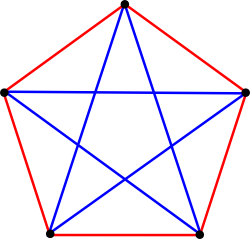
\includegraphics[width=0.4\columnwidth]{counter_example_R.png}
			\end{figure}\\
		\end{proof}
	\end{enumerate}
	